% -*- mode: latex; coding: utf-8 -*-

\section{Implementation}

\newthought{The results of this thesis} are an architecture for a software and
the software itself, written using the literate programming paradigm.

\subsection{Software architecture}

\newthought{Three aspects define the software architecture:}
\begin{enumerate*}
  \item an architectural software design pattern,
  \item layers and
  \item signals, allowing communication between components.
\end{enumerate*}
The used software design pattern uses four kinds of components as basis: models,
views, view models and controllers. It corresponds the model-view-view model
(MVVM) pattern but uses controllers additionally.
~\cref{fig:software-design-pattern-components} shows an overview of the
components (the colored items) including their communication. Additionally the
user as well as the display is shown (in gray color).

\begin{figure}[ht]
  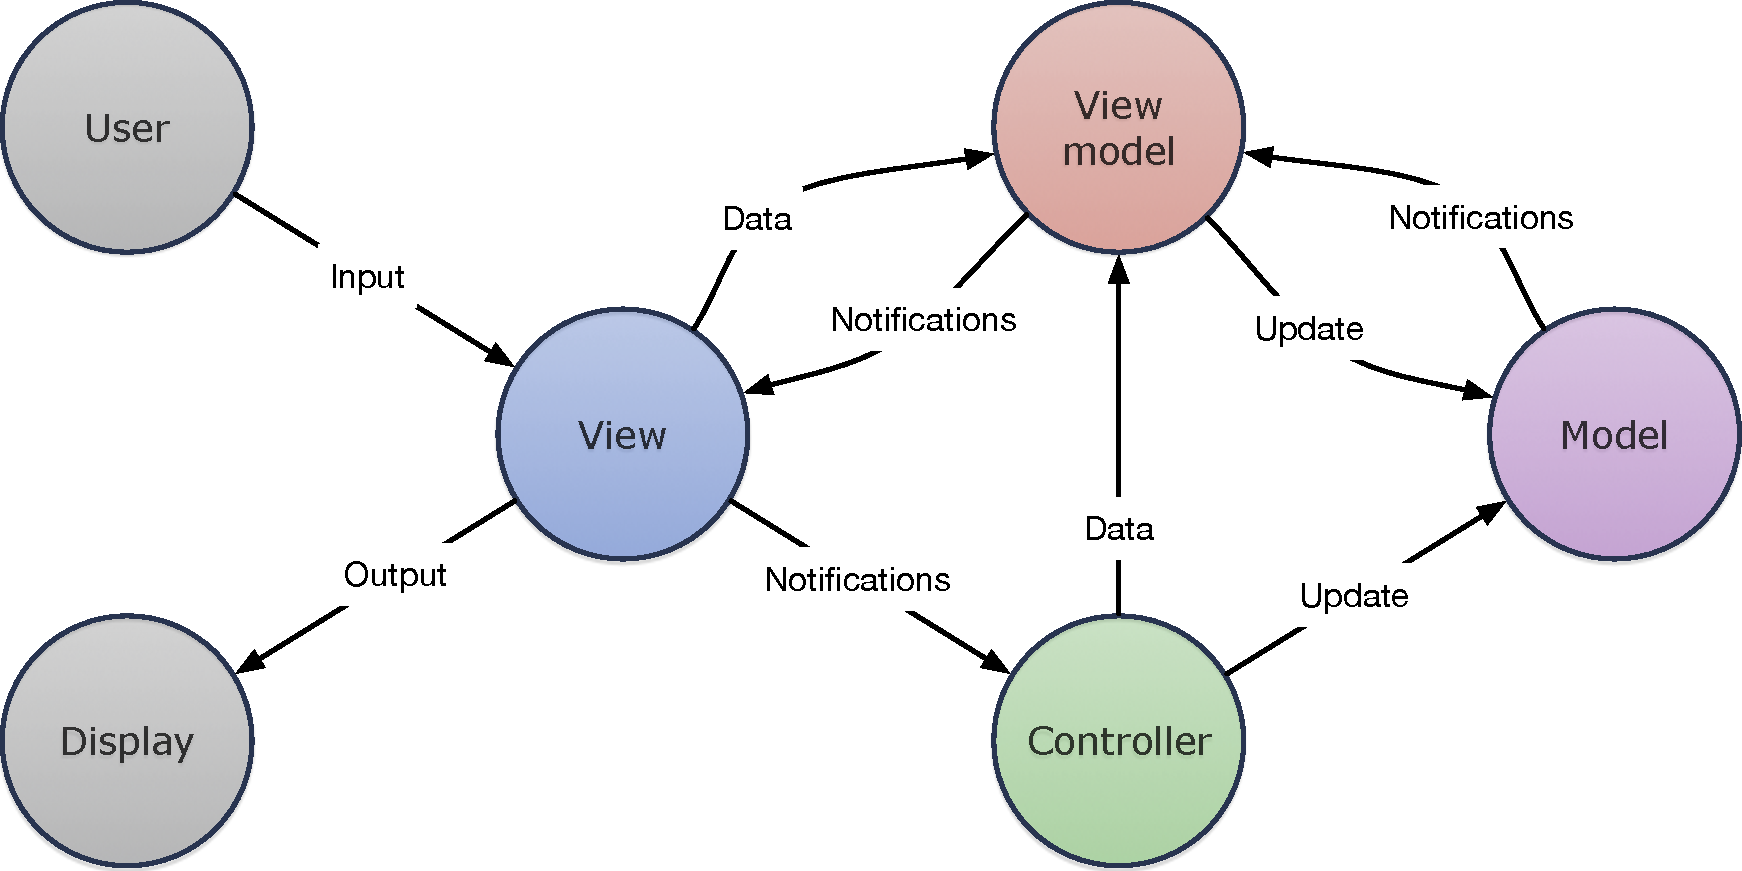
\includegraphics[width=0.8\linewidth]{images/mvvmc}
  \caption{Components of the used software design pattern and their communication.}
  \label{fig:software-design-pattern-components}
\end{figure}

\subsection{Software}

\newthought{The software itself} is an editor which allows \textit{modeling},
\textit{composing} and \textit{rendering} real time computer graphics through a
graphical toolbox. The editor was written in the python programming language
using the literate programming paradigm and uses the Qt framework as basis and
for the graphical user interface as well as OpenGL for rendering.

\newthought{Modeling} is done by composing single nodes to objects using a node
based graph structure. The basic nodes are defined by external files in JSON
notation. The graph structure allows adding, removing and connecting nodes to
complex objects. Every node has one ore more parameters, such as size or
position (of an object).

\newthought{Compositing} includes two aspects: the composition of objects into
scenes and the composition of an animation which is defined by multiple scenes
which follow a chronological order. The first aspect is realized by a scene
graph structure, which contains at least a root scene. Each scene may contain
objects in form of nodes which can be connected. The second aspect is realized
by a time line, which allows a chronological organization of scenes.

\newthought{For rendering} a highly optimized algorithm based on ray tracing is
used. The algorithm is called sphere tracing and allows the rendering of ray
traced scenes in real time on the GPU. Real-time means in this context being
able to generate at least 25 images in one second. Contingent upon the used
rendering algorithm all models are modeled using implicit surfaces.